% !TEX root = ../main.tex

\chapter{Python's ecosystem for scientific computing}

You can get your system ready installing the libraries with \texttt{pip}, Conda, your package manager or from source. 
\begin{codeblock}[language=bash]
# With pip 
pip install numpy scipy matplotlib pandas torch
\end{codeblock}




\section{Numpy}

NumPy is a core library for numerical computing in Python, offering an efficient interface for
working with arrays and matrices. Known for its high performance, it forms the basis of many other
scientific computing tools.
\begin{codeblock}[language=python]
import numpy as np
\end{codeblock}

\subsection{Arrays}
NumPy arrays provide an efficient way to store and manipulate numerical data, offering
advantages over traditional Python lists, particularly in terms of performance and functionality.

\subsubsection*{Creating arrays}
\begin{itemize}
    \item \textbf{From lists}:
    \begin{codeblock}[language=python]
    # 1D array
    a = np.array([1, 2, 3])

    # 2D array (matrix)
    b = np.array([[1, 2, 3], [4, 5, 6]])

    # Access the shape using the shape attribute
    print(a.shape)  # (3,)
    print(b.shape)  # (2, 3)
    \end{codeblock}

    Numpy arrays are faster and more memory efficient than Python lists. They also provide a lot of
    functionality for working with numerical data.
    The \texttt{dtype} attribute specifies the data type of the array.
    \begin{codeblock}[language=python]
    # Specify the data type
    c = np.array([1, 2, 3], dtype=np.float32)

    # Access the data type using the dtype attribute
    print(c.dtype)  # float32
    \end{codeblock}

    \item \textbf{Using array-generating functions}:
    \begin{codeblock}[language=python]
    # Create an array of zeros
    a = np.zeros((2, 3))

    # Create an array of ones
    b = np.ones((2, 3))

    # Using np.arange
    c = np.arange(0, 10, 2)

    # Using np.linspace
    d = np.linspace(0, 1, 5)
    \end{codeblock}

    \item \textbf{Reading from a file}:
    \begin{codeblock}[language=python]
    # Load data from a file
    data = np.genfromtxt('data.csv', delimiter=',')
    \end{codeblock}
\end{itemize}
    
\begin{observationblock}[Numpy arrays vs. Python lists]
    NumPy arrays offer several advantages over Python lists, such as:
    \begin{itemize}
        \item Faster access in reading and writing items.
        \item More convenient and efficient for mathematical operations.
        \item Occupying less memory.
    \end{itemize}
    Unlike Python lists, NumPy arrays are statically typed, homogeneous, memory-efficient, and support efficient mathematical operations implemented in compiled languages like C and Fortran.
\end{observationblock}

\subsubsection*{Array operations}

Array elements are accessed using square brackets and indices for reading and writing:
\begin{codeblock}[language=python]
a = np.array([1, 2, 3])
print(a[0])  # 1

a[0] = 5
print(a)  # [5, 2, 3]

b = np.array([[1, 2, 3], [4, 5, 6]])
print(b[0, 0])  # 1

b[0, 0] = 7
print(b)  # [[7, 2, 3], [4, 5, 6]]

# Slicing
print(a[1:])  # [2, 3]
print(b[1, :])  # [4, 5, 6]
\end{codeblock}

Numpy is well-suited for linear algebra operations, such as matrix multiplication:
\begin{codeblock}[language=python]
a = np.array([[1, 2], [3, 4]])
b = np.array([[5, 6], [7, 8]])

# Element-wise multiplication
print(a * b)

# Matrix multiplication
print(np.dot(a, b))
print(a @ b)

# Inverse and determinant
print(np.linalg.inv(a))
print(np.linalg.det(a))
\end{codeblock}

NumPy provides various functions to calculate statistics of datasets in arrays. Here are some
examples:
\begin{codeblock}[language=python]
a = np.array([[1, 2, 3], [4, 5, 6]])

# Mean
print(np.mean(a))

# Standard deviation
print(np.std(a))

# Sum
print(np.sum(a))

# Min and max
print(np.min(a))
print(np.max(a))
\end{codeblock}

When functions such as \texttt{min}, \texttt{max}, etc. are applied to multidimensional arrays, it is sometimes
useful to apply the calculation to the entire array or on a row or column basis. Using the \texttt{axis}
argument, we can specify how these functions should behave:
\begin{codeblock}[language=python]
a = np.array([[1, 2, 3], [4, 5, 6]])

# Column-wise minimum
print(np.min(a, axis=0))  # [1, 2, 3]

# Row-wise maximum
print(np.max(a, axis=1))  # [3, 6]

# Global max
print(np.max(a))  # 6
\end{codeblock}

\subsection{Reshaping, resizing and stacking arrays}

The shape of a NumPy array can be modified without copying the underlying data, making it a fast
operation even for large arrays:
\begin{codeblock}[language=python]
a = np.array([[1, 2, 3], [4, 5, 6]])

# Reshape
b = a.reshape(3, 2)
print(b)

# Flatten
c = a.flatten()
print(c)
\end{codeblock}

\begin{observationblock}
    Debug shapes before doing operations on matrices, it’s very easy to make mistakes and fuck up result shapes
\end{observationblock}

With \texttt{newaxis}, we can insert new dimensions in an array, for example converting a vector to a column or row matrix:
\begin{codeblock}[language=python]
a = np.array([1, 2, 3])

# Column vector
b = a[:, np.newaxis]
print(b)

# Row vector
c = a[np.newaxis, :]
print(c)
\end{codeblock}

Using functions \texttt{repeat}, \texttt{tile}, \texttt{vstack}, \texttt{hstack}, and \texttt{concatenate}, we can create larger
vectors and matrices from smaller ones:
\begin{codeblock}[language=python]
a = np.array([1, 2, 3])

# Repeat elements
b = np.repeat(a, 3)

# Tile elements
c = np.tile(a, 3)

# Stack arrays vertically
d = np.vstack([a, b])

# Stack arrays horizontally
e = np.hstack([a, b])

# Concatenate arrays
f = np.concatenate([a, b])
\end{codeblock}

\subsection{Linear Algebra}

To achieve high performance, assignments in Python usually do not copy the underlying objects.
This is important, for example, when objects are passed between functions to avoid an excessive
amount of memory copying when it is not necessary:
\begin{codeblock}[language=python]
a = np.array([1, 2, 3])
b = a

# Changing b will also change a
b[0] = 5
print(a)  # [5, 2, 3]
\end{codeblock}

Generally, we want to avoid iterating over the elements of arrays whenever possible. The Python
\texttt{for} loop is the most convenient way to iterate over an array when necessary:

\begin{codeblock}[language=python]
a = np.array([1, 2, 3])

for i in a:
    print(i)
\end{codeblock}

When we need to iterate over each element of an array and modify its elements, it is convenient to
use the \texttt{enumerate} function to obtain both the element and its index in the \texttt{for} loop:

\begin{codeblock}[language=python]
a = np.array([1, 2, 3])

for i, val in enumerate(a):
    a[i] = val * 2
\end{codeblock}

As mentioned several times, to achieve good performance, we should avoid looping over
elements in our vectors and matrices and instead use vectorized algorithms. The first step is to
make sure that functions work with vector inputs:

\begin{codeblock}[language=python]
def my_func(x):
    if x > 0:
        return x ** 2
    else:
        return x / 2

# This will raise an error
# my_func(np.array([-1, 2, 3]))

# Instead, use np.vectorize
my_vec_func = np.vectorize(my_func)
print(my_vec_func(np.array([-1, 2, 3])))
\end{codeblock}

When using arrays in conditions, for example \texttt{if} statements and other boolean expressions, use
\texttt{any} or \texttt{all} , requiring that any or all elements in the array evaluate to \texttt{True} :

\begin{codeblock}[language=python]
a = np.array([True, False, True])

# Check if any element is True
print(np.any(a))

# Check if all elements are True
print(np.all(a))
\end{codeblock}

Since NumPy arrays are statically typed, the type of an array does not change once created. But
we can explicitly cast an array of some type to another using the \texttt{astype} functions (see also the
similar \texttt{asarray} function). This always creates a new array of new type:

\begin{codeblock}[language=python]
a = np.array([1, 2, 3], dtype=np.float32)

# Cast to int32
b = a.astype(np.int32)
\end{codeblock}



\section{Scipy}

SciPy, built on NumPy's foundation, offers higher-level scientific algorithms and modules for
specialized tasks like optimization, integration, signal processing, and linear algebra. It provides
seamless interoperability with NumPy for efficient data representation and manipulation.

To access the SciPy package in a Python program, we start by importing everything from the
\texttt{scipy} module:
\begin{codeblock}[language=python]
import scipy as sp
\end{codeblock}

\subsubsection*{Numerical integration}

For the numerical evaluation of a definite integral of the type 
\[
\int_{a}^{b} f(x) \, dx
\]
we can use the \texttt{quad} function from the \texttt{scipy.integrate} module. The function takes as input the
function to integrate, the lower and upper limits of integration, and returns the integral value and an estimate of the error:

\begin{codeblock}[language=python]
from scipy.integrate import quad

def f(x):
    return x ** 2

result, error = quad(f, 0, 1)
print(result)  # 0.33333333333333337
print(error)  # 3.700743415417189e-15
\end{codeblock}

Higher dimensional integrals can be evaluated using the \texttt{nquad} function, which takes a list of functions and a list of integration limits:

\begin{codeblock}[language=python]
from scipy.integrate import nquad

def f(x, y):
    return x * y

result, error = nquad(f, [[0, 1], [0, 1]])
print(result)  # 0.25
print(error)  # 2.7755575615628914e-15
\end{codeblock}

\subsubsection*{ODEs}

A system of ODEs is usually formulated in standard form before it is attacked numerically. The
standard form is
\[
\frac{d\mathbf{y}}{dt} = \mathbf{f}(\mathbf{y}, t)
\]
where $\mathbf{y}$ is the vector of dependent variables and $\mathbf{f}$ is the vector of right-hand sides of the ODEs. 
SciPy provides two different ways to solve ODEs: an API based on the function \texttt{odeint} and an
object-oriented API based on the class \texttt{ode}. Usually, \texttt{odeint} is easier to get started with, but the
\texttt{ode} class offers some finer level of control.
The SciPy function \texttt{odeint} solves the initial value problem for a system of ODEs:

\begin{codeblock}[language=python]
from scipy.integrate import odeint

def f(y, t):
    return -y

y0 = 1
t = np.linspace(0, 10, 100)
y = odeint(f, y0, t)
\end{codeblock}

\subsubsection*{Fourier transforms}

SciPy's \texttt{fft} module enables easy computation of Fourier transforms, a critical tool in
computational physics, signal processing and data analysis.

\begin{codeblock}[language=python]
from scipy.fft import fft, ifft
import numpy as np

N = 600 # Number of sample points
T = 1.0 / 800.0 # sample spacing

x = np.linspace(0.0, N*T, N, endpoint=False)
y = np.sin(50.0 * 2.0 * np.pi * x) + 0.5 * np.sin(80.0 * 2.0 * np.pi * x)

yf = fft(y)
xf = fftfreq(N, T)[:N//2]
\end{codeblock}

\subsubsection*{Linear Algebra}

The linear algebra module contains various matrix-related functions, including linear equation
solving, eigenvalue solvers, matrix functions (e.g., matrix exponentiation), decompositions (SVD,
LU, Cholesky), etc.

\begin{codeblock}[language=python]
from scipy.linalg import solve, inv

A = np.array([[1, 2], [3, 4]])
b = np.array([1, 2])

x = solve(A, b)
print(x)  # [-1. ,  1.5]

A_inv = inv(A)
print(A_inv)

# Eigenvalues and eigenvectors
eigvals, eigvecs = np.linalg.eig(A)
print(eigvals)
print(eigvecs)
\end{codeblock}

Sparse matrices are often useful in numerical simulations dealing with large systems, where the
problem can be described in matrix form, and matrices or vectors mostly contain zeros. SciPy has
good support for sparse matrices, with basic linear algebra operations (e.g., equation solving,
eigenvalue calculations, etc.).

There are many possible strategies for storing sparse matrices efficiently, such as coordinate form
(COO), list of lists (LIL) form, and compressed-sparse column CSC (and row, CSR). Each format
has some advantages and disadvantages. Most computational algorithms (equation solving,
matrix-matrix multiplication, etc.) can be efficiently implemented using CSR or CSC formats, but
they are not so intuitive and not so easy to initialize. So often, a sparse matrix is initially created in
COO or LIL format (where we can efficiently add elements to the sparse matrix data), and then
converted to CSC or CSR before used in real calculations.

\begin{codeblock}[language=python]
from scipy.sparse import csr_matrix

# Create a sparse matrix
data = np.array([1, 2, 3, 4])
row = np.array([0, 0, 1, 1])
col = np.array([0, 1, 0, 1])

A = csr_matrix((data, (row, col)), shape=(2, 2))
print(A.toarray())

# Create a dense matrix
B = np.array([[1, 2], [3, 4]])

# Convert to sparse matrix
C = csr_matrix(B)
\end{codeblock}

\subsubsection*{Optimization}

Optimization (finding minima or maxima of a function) is a large field in mathematics, and
optimization of complicated functions or in many variables can be rather involved.

\begin{codeblock}[language=python]
from scipy.optimize import optimize 

def f(x):
    return x ** 2

result = optimize.fmin_bfgs(f, x0=0)
\end{codeblock}

To find the roots of a function of the form $f(x) = 0$, we can use the \texttt{fsolve} function. It requires an initial guess for the root:

\begin{codeblock}[language=python]
from scipy.optimize import fsolve

def f(x):
    return x ** 2 - 2

result = fsolve(f, x0=0)
\end{codeblock}

\subsubsection*{Interpolation}

The \texttt{interp1d} function, when given arrays describing X and Y data, returns an object that
behaves like a function that can be called for an arbitrary value of x (in the range covered by X),
and it returns the corresponding interpolated y value:

\begin{codeblock}[language=python]
from scipy.interpolate import interp1d

x = np.linspace(0, 10, 10)
y = np.sin(x)

f = interp1d(x, y)
print(f(5))
\end{codeblock}

\subsubsection*{Statistics}

The \texttt{scipy.stats} module contains a large number of probability distributions as well as a growing library of statistical functions.

\begin{codeblock}[language=python]
from scipy.stats import norm

# Create a normal distribution
dist = norm(loc=0, scale=1)

# Calculate the probability density function
print(dist.pdf(0))

# Calculate the cumulative distribution function
print(dist.cdf(0))

# Generate random numbers
print(dist.rvs(10))
\end{codeblock}

SciPy includes functions for conducting statistical tests, like t-tests and ANOVA, aiding in
hypothesis testing and data analysis.

Calculate the T-test for the means of two independent samples:
\begin{codeblock}[language=python]
    t_statistic, p_value = stats.ttest_ind(X.rvs(1000), Y.rvs(1000))
\end{codeblock}

Test if the mean of a single sample of data is 0.1:
\begin{codeblock}[language=python]
    stats.ttest_1samp(Y.rvs(size = 1000), 0.1)
\end{codeblock}








\section{Data Visualization}

Data visualization plays a vital role in data analysis, enabling the effective communication of
complex information. Matplotlib and Seaborn are two widely-used Python libraries for data
visualization. Matplotlib offers a wide range of plotting tools, while Seaborn provides a high-level
interface for drawing attractive statistical graphics.

\subsection{Matplotlib}

Matplotlib is a widely-used 2D plotting library in Python. It provides a high-level interface for
drawing attractive and informative statistical graphics. Let's start with a simple example to create a
basic line plot:

\begin{codeblock}[language=python]
    import matplotlib.pyplot as plt
    import numpy as np

    # Generate data.
    x = np.linspace(0, 10, 100)
    y = np.sin(x)

    # Create simple plots.
    plt.plot(x, y, label='sin(x)') # line plot
    # plt.scatter(x,y, label = 'sin(x)') # scatter plot
    plt.title('Simple line plot')
    plt.xlabel('x-axis')
    plt.ylabel('y-axis')
    plt.legend()
    plt.show()
\end{codeblock}

\begin{figure}[H]
    \centering
    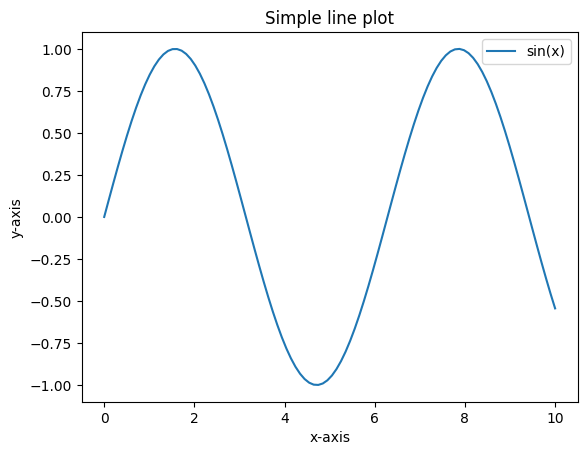
\includegraphics[width=0.7\textwidth]{assets/fig1_mpl.png}
    \caption{A simple line plot using Matplotlib.}
\end{figure}

In this example, we use NumPy to generate data points for the x-axis and calculate corresponding
y-values. The \texttt{plot} function is then used to create a line plot. Finally, \texttt{title} , \texttt{xlabel} , \texttt{ylabel} ,
and \texttt{legend} functions are used to add a title, axis labels, and a legend to the plot.
Matplotlib supports various types of plots, including scatter plots, bar plots, histograms, and more.
Explore the documentation for more plot types and customization options.

Let's create a 2D contour plot using Matplotlib.
\begin{codeblock}[language=python]
    import matplotlib.pyplot as plt
    import numpy as np

    # Generate data.
    x = np.linspace(-5, 5, 100)
    y = np.linspace(-5, 5, 100)
    X, Y = np.meshgrid(x, y)
    Z = np.sin(np.sqrt(X**2 + Y**2))

    # Create a 2D contour plot.
    plt.contourf(X, Y, Z, cmap='viridis')
    plt.colorbar(label='sin(sqrt(x^2 + y^2))')
    plt.title('Contour plot')
    plt.xlabel('x-axis')
    plt.ylabel('y-axis')
    plt.show()
\end{codeblock}

\begin{figure}[H]
    \centering
    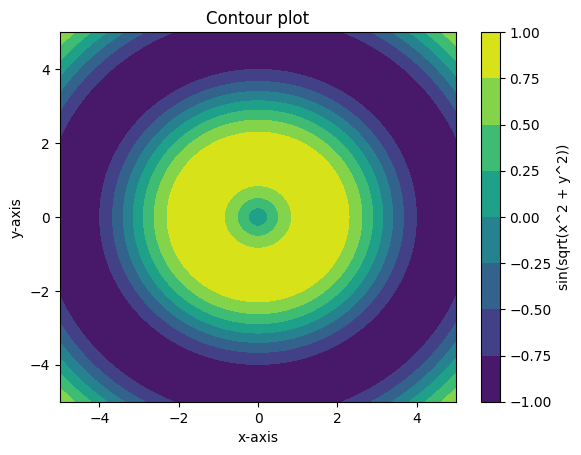
\includegraphics[width=0.7\textwidth]{assets/fig2_mpl.png}
    \caption{A 2D contour plot using Matplotlib.}
\end{figure}

\subsection{Seaborn}

Seaborn, built on Matplotlib, provides a more intuitive interface for creating statistical plots. It
integrates well with pandas data structures and offers built-in themes for enhanced visual appeal.

\begin{codeblock}[language=python]
    import seaborn as sns
    import numpy as np
    # Generate data.
    x = np.random.randn(100)
    y = 2 * x + np.random.randn(100)
    # Create a scatter plot using Seaborn.
    sns.scatterplot(x=x, y=y, color='blue')
    plt.title('Scatter Plot with Seaborn')
    plt.xlabel('x-axis')
    plt.ylabel('y-axis')
    plt.show()
\end{codeblock}

\begin{figure}[H]
    \centering
    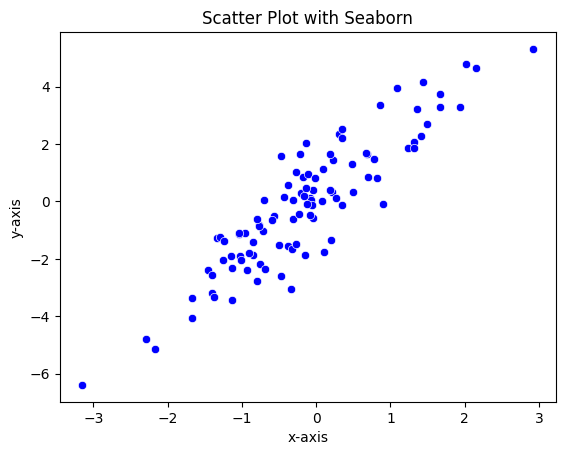
\includegraphics[width=0.7\textwidth]{assets/fig3_mpl.png}
    \caption{A scatter plot using Seaborn.}
\end{figure}

Let's create a customized histogram with Seaborn, including specific bin edges, colors, and
additional statistical annotations.

\begin{codeblock}[language=python]
    import seaborn as sns
    import numpy as np
    # Generate data.
    x = np.random.randn(100)
    # Create a histogram using Seaborn.
    sns.histplot(x, bins=[-3, -2, -1, 0, 1, 2, 3], color='green', kde=True)
    plt.title('Histogram with Seaborn')
    plt.xlabel('x-axis')
    plt.ylabel('Frequency')
    plt.show()
\end{codeblock}

\begin{figure}[H]
    \centering
    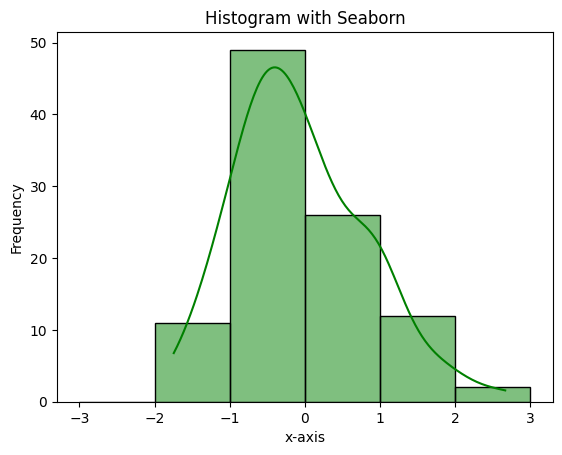
\includegraphics[width=0.7\textwidth]{assets/fig4_mpl.png}
    \caption{A histogram using Seaborn.}
\end{figure}

One of the strengths of Seaborn is its ability to work seamlessly with Matplotlib. You can use
Matplotlib functions alongside Seaborn to customize your plots further. Here's an example
combining Matplotlib and Seaborn to create a histogram with a kernel density estimate:

\begin{codeblock}[language=python]
    import seaborn as sns
    import numpy as np
    # Generate data.
    x = np.random.randn(100)
    # Create a histogram with KDE using Seaborn.
    sns.histplot(x, bins=20, color='red', kde=True)
    plt.title('Histogram with KDE using Seaborn')
    plt.xlabel('x-axis')
    plt.ylabel('Frequency')
    plt.show()
\end{codeblock}

\begin{figure}[H]
    \centering
    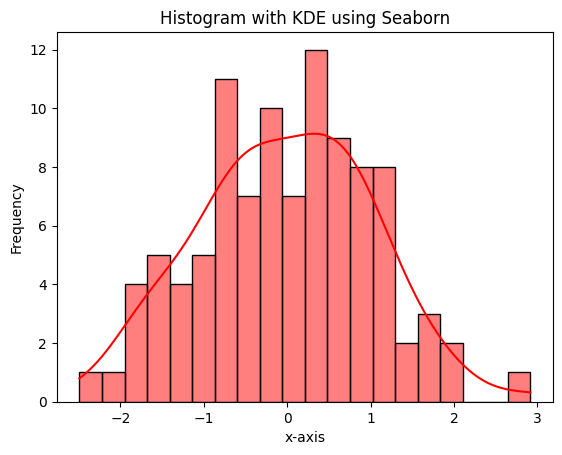
\includegraphics[width=0.7\textwidth]{assets/fig5_mpl.png}
    \caption{A histogram with KDE using Seaborn.}
\end{figure}

Matplotlib supports advanced plots like contour plots, 3D plots, and subplots:
\begin{itemize}
    \item Contour plots for visualizing three-dimensional data.
    \item Subplots for displaying multiple plots in a single figure.
\end{itemize}

Seaborn excels in creating complex statistical plots:
\begin{itemize}
    \item Heatmaps for representing matrix data.
    \item Pair plots for exploring relationships in a dataset.
    \item Facet grids for plotting subsets of data on multiple axes.
\end{itemize}
Matplotlib and Seaborn can directly plot from pandas DataFrame, simplifying the workflow in data
analysis tasks.



\section{Pandas}

pandas is a powerful Python library for data manipulation and analysis. It provides fast, flexible
data structures like Series and DataFrame, designed to work with structured data intuitively and
efficiently.

In the pandas library, the standard import convention involves using the aliases \texttt{np} for NumPy and \texttt{pd} for pandas:

\begin{codeblock}[language=python]
    import numpy as np
    import pandas as pd
\end{codeblock}

\subsection{Overview}

The fundaental structures are:
\begin{itemize}
    \item \textbf{Series}: A one-dimensional array-like object containing an array of data and an associated array of data labels, called an index.
    \item \textbf{DataFrame}: A two-dimensional tabular data structure with labeled axes (rows and columns).
\end{itemize}

To create a Series, pass a list of values to the \texttt{pd.Series} constructor. By default, pandas will create an index starting from 0:

\begin{codeblock}[language=python]
    # Create a Series
    s = pd.Series([1, 3, 5, np.nan, 6, 8])

    # Create a DataFrame
    dates = pd.date_range('20210101', periods=6)
    df = pd.DataFrame(np.random.randn(6, 4), index=dates, columns=list('ABCD'))
\end{codeblock}

We can also view the top and bottom rows of the DataFrame using the \texttt{head} and \texttt{tail} methods:

\begin{codeblock}[language=python]
    print(df.head())
    print(df.tail())
\end{codeblock}
 
or retrieve the index, columns, and underlying NumPy data:

\begin{codeblock}[language=python]
    print(df.index)
    print(df.columns)
    print(df.values)
\end{codeblock}

\begin{observationblock}
    \textbf{NumPy arrays have one dtype for the entire array while pandas DataFrames have one
    dtype per column.} When you call \plaintt{DataFrame.to\_numpy()}, pandas will find the NumPy dtype
    that can hold all of the dtypes in the DataFrame. If the common data type is \plaintt{object}, \plaintt{DataFrame.to\_numpy()} will require copying data.
\end{observationblock}

pandas offers various methods for data selection. For a DataFrame, passing a single label selects a columns and yields a Series equivalent to
\texttt{df.A}:

\begin{codeblock}[language=python]
    print(df['A'])
\end{codeblock}

Passing a slice \texttt{:} selects rows:

\begin{codeblock}[language=python]
    print(df[0:3])
\end{codeblock}

\begin{itemize}
    \item \textbf{Selection by label}: For getting a cross-section using a label, use the \texttt{.loc} method.
    \begin{codeblock}[language=python]
        print(df.loc[dates[0]])
    \end{codeblock}
    \item \textbf{Selection by position}: For selecting via the position of the passed integers, use the \texttt{.iloc} method.
    \begin{codeblock}[language=python]
        print(df.iloc[3])
    \end{codeblock}
\end{itemize}

Generate quick statistics using the \texttt{describe} method:

\begin{codeblock}[language=python]
    print(df.describe())
\end{codeblock}

Transpose the DataFrame using the \texttt{T} attribute:

\begin{codeblock}[language=python]
    print(df.T)
\end{codeblock}

Sort the DataFrame by index or value:

\begin{codeblock}[language=python]
    print(df.sort_index(axis=1, ascending=False))
    print(df.sort_values(by='B'))
\end{codeblock}

\subsubsection*{Operations}

Perform statistical operations like mean, median, and sum on the DataFrame:

\begin{codeblock}[language=python]
    print(df.mean())
    print(df.median())
    print(df.sum())
\end{codeblock}

Perform operations with another DataFrame or Series:

\begin{codeblock}[language=python]
    s = pd.Series([1, 3, 5, np.nan, 6, 8], index=dates).shift(2)
    print(df.sub(s, axis='index'))
\end{codeblock}

Apply user-defined functions to the DataFrame using \texttt{agg} or \texttt{transform} methods:

\begin{codeblock}[language=python]
    # Apply a function to the DataFrame
    print(df.agg(np.sum))

    # Apply a function to each column
    print(df.transform(lambda x: x * 2))
\end{codeblock}

Compute value counts for a Series:

\begin{codeblock}[language=python]
    s = pd.Series(['A', 'B', 'C', 'A', 'B', 'C', 'A', 'A', 'B'])
    print(s.value_counts())
\end{codeblock}

pandas simplifies handling missing values using the \texttt{dropna}, \texttt{fillna}, and \texttt{isna} methods:

\begin{codeblock}[language=python]
    # Drop rows with missing values
    print(df.dropna())

    # Fill missing values with a constant
    print(df.fillna(value=0))

    # Check for missing values
    print(df.isna())
\end{codeblock}

pandas also integrates with Matplotlib and Seaborn for data visualization. For example, we can
create a line plot of the DataFrame using the \texttt{plot} method:

\begin{codeblock}[language=python]
    df.plot()
    plt.show()
\end{codeblock}

\subsubsection*{Importing and Exporting data}

pandas supports reading and writing data in various formats, including CSV, Excel, SQL, and more.
To read a CSV file into a DataFrame, use the \texttt{read\_csv} method:

\begin{codeblock}[language=python]
    df = pd.read_csv('data.csv')
\end{codeblock}


\section{PyTorch}

PyTorch is a Python-based scientific computing package serving two broad purposes:
\begin{itemize}
    \item A replacement for NumPy to use the power of GPUs.
    \item A deep learning research platform that provides maximum flexibility and speed.
\end{itemize}

The package is imported as follows:

\begin{codeblock}[language=python]
    import torch
\end{codeblock}

\subsection*{Tensors}

Tensors are the PyTorch equivalent to Numpy arrays, with the addition to also have support for GPU acceleration.
In multilinear algebra, tensor is a generalization of vector and matrix concepts:
\begin{itemize}
    \item A scalar is a 0-dimensional tensor.
    \item A vector is a 1-dimensional tensor.
    \item A matrix is a 2-dimensional tensor.
\end{itemize}

A tensor can be simply initialized using the \texttt{torch.tensor} function:

\begin{codeblock}[language=python]
    # Create a tensor
    x = torch.tensor([1, 2, 3])
    print(x)
\end{codeblock}

The function \texttt{torch.Tensor} allocates memory for the desired tensor, but reuses any values that
have already been in the memory. To directly assign values to the tensor during initialization, there
are many alternatives including:
\begin{itemize}
    \item \texttt{torch.zeros} to initialize a tensor of zeros.
    \item \texttt{torch.ones} to initialize a tensor of ones.
    \item \texttt{torch.rand} to initialize a tensor with random values.
\end{itemize}

\begin{codeblock}[language=python]
    # Create a tensor of zeros
    x = torch.zeros(2, 3)
    print(x)

    # Create a tensor of ones
    y = torch.ones(2, 3)
    print(y)

    # Create a tensor with random values
    z = torch.rand(2, 3)
    print(z)
\end{codeblock}

\begin{observationblock}
    PyTorch tensors are similar to NumPy arrays, but with additional support for GPU acceleration. They can be easily converted to and from NumPy arrays using the \plaintt{torch.from\_numpy} and \plaintt{.numpy()} methods.
\end{observationblock}

\subsection*{Operations}

PyTorch tensors support a wide range of operations, similar to NumPy arrays. Here are some examples:

\begin{codeblock}[language=python]
    x = torch.tensor([1, 2, 3])
    y = torch.tensor([4, 5, 6])

    # Element-wise addition
    z = x + y
    print(z)

    # Element-wise multiplication
    z = x * y
    print(z)

    # Matrix multiplication
    x = torch.tensor([[1, 2], [3, 4]])
    y = torch.tensor([[5, 6], [7, 8]])
    z = torch.mm(x, y)
    print(z)
\end{codeblock}

Other commonly used operations include matrix multiplications, which are essential for neural
networks:
\begin{itemize}
    \item \texttt{torch.mm} for matrix multiplication.
    \item \texttt{torch.bmm} for batch matrix multiplication. If the first tensor T is of shape (b, n, m) and the second tensor is of shape (b, m, p), the result will be a tensor of shape (b, n, p).
    \item \texttt{torch.matmul} for matrix multiplication with broadcasting.
\end{itemize}

\subsection*{Dynamic Computation Graphs}

One of the main reasons for using PyTorch in Deep Learning projects is that we can automatically
get gradients/derivatives of functions that we define.
We will mainly use PyTorch for implementing neural networks, and they are just fancy functions. If
we use weight matrices in our function that we want to learn, then those are called the
\textbf{parameters} or simply the \textbf{weights}.

Given an input \texttt{x}, we define our function by manipulating that input, usually by matrix-
multiplications with weight matrices and additions with so-called bias vectors. As we manipulate
our input, we are automatically creating a computational graph.

This graph shows how to arrive at our output from our input. PyTorch is a \textbf{define-by-run}
framework; this means that we can just do our manipulations, and PyTorch will keep track of that
graph for us. Thus, we create a dynamic computation graph along the way.

Let's compute the computational graph for a function:
\[ 
y = \frac{1}{l(x)}\sum_{i}^{}[(x_i + 2)^2 + 3]
\]

\begin{codeblock}[language=python]
    x = torch.arange(3, dtype=torch.float32, requires_grad=True)
    # Only float tensors can have gradients
    # X tensor([0., 1., 2.], requires_grad=True)

    a = x + 2
    b = a ** 2
    c = b + 3
    y = c.mean()
    print("Y", y)
    # Y tensor(12.6667, grad_fn=<MeanBackward0>)
\end{codeblock}

We can perform backpropagation on the computation graph by calling the \texttt{backward()} function on the last output, which effectively calculates the gradients for each tensor that has the property
\texttt{requires\_grad=True}:

\begin{codeblock}[language=python]
    y.backward()
    print(x.grad)
    # X.grad tensor([1.3333, 2.6667, 4.], requires_grad=True)
\end{codeblock}

\subsection*{GPU support}

A crucial feature of PyTorch is the support of GPUs, short for Graphics Processing Unit. A GPU
can perform many thousands of small operations in parallel, making it very well suitable for
performing large matrix operations in neural networks.
To check if we have a GPU available:

\begin{codeblock}[language=python]
    gpu_available = torch.cuda.is_available()
    print(gpu_available)
\end{codeblock}

You can write your code with respect to this device object, and it allows you to run the same code
on both a CPU-only system, and one with a GPU. Let’s try it below. We can specify the device as
follows:

\begin{codeblock}[language=python]
    device = torch.device('cuda' if torch.cuda.is_available() else 'cpu')
    print(device)
\end{codeblock}

\subsection*{Designing Neural Networks}

The package \texttt{torch.nn} is the heart of PyTorch. It provides the building blocks for designing and training neural networks. The key components are:

\begin{itemize}
    \item \textbf{Module}: A neural network layer. It can be a single layer, a collection of layers, or a complete neural network.
    \item \textbf{Sequential}: A container for Modules that are executed in order.
    \item \textbf{Loss Function}: A function that measures the difference between the predicted output and the target output.
    \item \textbf{Optimizer}: A function that adjusts the weights of the neural network to minimize the loss function.
\end{itemize}

The easiest way to create a neural network in PyThorch is with \textbf{Modules}:

\begin{codeblock}[language=python]
    import torch.nn as nn

    class NeuralNetwork(nn.Module):
        def __init__(self):
            super(NeuralNetwork, self).__init__()
            self.layer1 = nn.Linear(10, 5)
            self.layer2 = nn.Linear(5, 1)

        def forward(self, x):
            x = self.layer1(x)
            x = self.layer2(x)
            return x
\end{codeblock}

The class \texttt{torch.utils.data.DataLoader} represents a Python iterable over a dataset with
support for automatic batching, multi-process data loading and many more features. The data
loader communicates with the dataset using the function \texttt{\_\_getitem\_\_}, and stacks its outputs as
tensors over the first dimension to form a batch. In contrast to the dataset class, we usually don’t
have to define our own data loader class, but can just create an object of it with the dataset as
input. Additionally, we can configure our data loader with the following input arguments (only a
selection, see full list here):
\begin{itemize}
    \item \texttt{batch\_size}: The number of samples in a batch.
    \item \texttt{shuffle}: If the data should be shuffled at every epoch.
    \item ...
\end{itemize}

After defining the model and the dataset, it is time to prepare the optimization of the model. During
training, we will perform the following steps:

\begin{itemize}
    \item Forward pass: Compute the predicted output.
    \item Compute the loss: Compute the difference between the predicted output and the target output.
    \item Backward pass: Compute the gradients of the loss with respect to the model parameters.
    \item Update the weights: Adjust the weights of the model to minimize the loss.
\end{itemize}

We can calculate the loss for a batch by simply performing a few tensor operations as those are
automatically added to the computation graph. For instance, for regression we can use Mean
Squared Error (MSE) which is defined as
\[
\text{MSE} = \frac{1}{n}\sum_{i=1}^{n}(y_i - \hat{y}_i)^2
\]
where $y_i$ is the true value and $\hat{y}_i$ is the predicted value.

For updating the parameters of the model, we can use the \texttt{torch.optim} package. It provides a
wide range of optimization algorithms, including SGD, Adam, and RMSprop. The optimizer takes the model parameters and the learning rate as input:

\begin{codeblock}[language=python]
    import torch.optim as optim

    model = NeuralNetwork()
    optimizer = optim.SGD(model.parameters(), lr=0.01)
\end{codeblock}

